% Created 2020-04-15 三 14:46
% Intended LaTeX compiler: pdflatex
\documentclass[11pt]{article}
\usepackage[utf8]{inputenc}
\usepackage[T1]{fontenc}
\usepackage{graphicx}
\usepackage{grffile}
\usepackage{longtable}
\usepackage{wrapfig}
\usepackage{rotating}
\usepackage[normalem]{ulem}
\usepackage{amsmath}
\usepackage{textcomp}
\usepackage{amssymb}
\usepackage{capt-of}
\usepackage{imakeidx}
\usepackage{hyperref}
\usepackage{minted}
% TIPS
% \substack{a\\b} for multiple lines text





% pdfplots will load xolor automatically without option
\usepackage[dvipsnames]{xcolor}

\usepackage{forest}
% two-line text in node by [two \\ lines]
% \begin{forest} qtree, [..] \end{forest}
\forestset{
  qtree/.style={
    baseline,
    for tree={
      parent anchor=south,
      child anchor=north,
      align=center,
      inner sep=1pt,
    }}}
%\usepackage{flexisym}
% load order of mathtools and mathabx, otherwise conflict overbrace

\usepackage{mathtools}
%\usepackage{fourier}
\usepackage{pgfplots}
\usepackage{amsthm}
\usepackage{amsmath}
%\usepackage{unicode-math}
%
\usepackage{commath}
%\usepackage{,  , }
\usepackage{amsfonts}
\usepackage{amssymb}
% importing symbols https://tex.stackexchange.com/questions/14386/importing-a-single-symbol-from-a-different-font
%mathabx change every symbol
% use instead stmaryrd
%\usepackage{mathabx}
\usepackage{stmaryrd}
\usepackage{empheq}
\usepackage{tikz}
\usepackage{tikz-cd}
%\usepackage[notextcomp]{stix}
\usetikzlibrary{arrows.meta}
\usepackage[most]{tcolorbox}
%\utilde
%\usepackage{../../latexpackage/undertilde/undertilde}
% left and right superscript and subscript
\usepackage{actuarialsymbol}
\usepackage{threeparttable}
\usepackage{scalerel,stackengine}
\usepackage{stackrel}
% \stackrel[a]{b}{c}
\usepackage{dsfont}
% text font
\usepackage{newpxtext}
%\usepackage{newpxmath}

%\newcounter{dummy} \numberwithin{dummy}{section}
\newtheorem{dummy}{dummy}[section]
\theoremstyle{definition}
\newtheorem{definition}[dummy]{Definition}
\newtheorem{corollary}[dummy]{Corollary}
\newtheorem{lemma}[dummy]{Lemma}
\newtheorem{proposition}[dummy]{Proposition}
\newtheorem{theorem}[dummy]{Theorem}
\theoremstyle{definition}
\newtheorem{example}[dummy]{Example}
\theoremstyle{remark}
\newtheorem*{remark}{Remark}


\newcommand\what[1]{\ThisStyle{%
    \setbox0=\hbox{$\SavedStyle#1$}%
    \stackengine{-1.0\ht0+.5pt}{$\SavedStyle#1$}{%
      \stretchto{\scaleto{\SavedStyle\mkern.15mu\char'136}{2.6\wd0}}{1.4\ht0}%
    }{O}{c}{F}{T}{S}%
  }
}

\newcommand\wtilde[1]{\ThisStyle{%
    \setbox0=\hbox{$\SavedStyle#1$}%
    \stackengine{-.1\LMpt}{$\SavedStyle#1$}{%
      \stretchto{\scaleto{\SavedStyle\mkern.2mu\AC}{.5150\wd0}}{.6\ht0}%
    }{O}{c}{F}{T}{S}%
  }
}

\newcommand\wbar[1]{\ThisStyle{%
    \setbox0=\hbox{$\SavedStyle#1$}%
    \stackengine{.5pt+\LMpt}{$\SavedStyle#1$}{%
      \rule{\wd0}{\dimexpr.3\LMpt+.3pt}%
    }{O}{c}{F}{T}{S}%
  }
}

\newcommand{\bl}[1] {\boldsymbol{#1}}
\newcommand{\Wt}[1] {\stackrel{\sim}{\smash{#1}\rule{0pt}{1.1ex}}}
\newcommand{\wt}[1] {\widetilde{#1}}
\newcommand{\tf}[1] {\textbf{#1}}


%For boxed texts in align, use Aboxed{}
%otherwise use boxed{}

\DeclareMathSymbol{\widehatsym}{\mathord}{largesymbols}{"62}
\newcommand\lowerwidehatsym{%
  \text{\smash{\raisebox{-1.3ex}{%
    $\widehatsym$}}}}
\newcommand\fixwidehat[1]{%
  \mathchoice
    {\accentset{\displaystyle\lowerwidehatsym}{#1}}
    {\accentset{\textstyle\lowerwidehatsym}{#1}}
    {\accentset{\scriptstyle\lowerwidehatsym}{#1}}
    {\accentset{\scriptscriptstyle\lowerwidehatsym}{#1}}
}

\usepackage{graphicx}
    
% text on arrow for xRightarrow
\makeatletter
%\newcommand{\xRightarrow}[2][]{\ext@arrow 0359\Rightarrowfill@{#1}{#2}}
\makeatother


\newcommand{\dom}[1]{%
\mathrm{dom}{(#1)}
}

% Roman numerals
\makeatletter
\newcommand*{\rom}[1]{\expandafter\@slowromancap\romannumeral #1@}
\makeatother

\def \fR {\mathfrak{R}}
\def \bx {\boldsymbol{x}}
\def \bz {\boldsymbol{z}}
\def \ba {\boldsymbol{a}}
\def \bh {\boldsymbol{h}}
\def \bo {\boldsymbol{o}}
\def \bU {\boldsymbol{U}}
\def \bc {\boldsymbol{c}}
\def \bV {\boldsymbol{V}}
\def \bI {\boldsymbol{I}}
\def \bK {\boldsymbol{K}}
\def \bt {\boldsymbol{t}}
\def \bb {\boldsymbol{b}}
\def \bA {\boldsymbol{A}}
\def \bX {\boldsymbol{X}}
\def \bu {\boldsymbol{u}}
\def \bS {\boldsymbol{S}}
\def \bZ {\boldsymbol{Z}}
\def \bz {\boldsymbol{z}}
\def \by {\boldsymbol{y}}
\def \bw {\boldsymbol{w}}
\def \bT {\boldsymbol{T}}
\def \bF {\boldsymbol{F}}
\def \bS {\boldsymbol{S}}
\def \bm {\boldsymbol{m}}
\def \bW {\boldsymbol{W}}
\def \bR {\boldsymbol{R}}
\def \bQ {\boldsymbol{Q}}
\def \bS {\boldsymbol{S}}
\def \bP {\boldsymbol{P}}
\def \bT {\boldsymbol{T}}
\def \bY {\boldsymbol{Y}}
\def \bH {\boldsymbol{H}}
\def \bB {\boldsymbol{B}}
\def \blambda {\boldsymbol{\lambda}}
\def \bPhi {\boldsymbol{\Phi}}
\def \btheta {\boldsymbol{\theta}}
\def \bTheta {\boldsymbol{\Theta}}
\def \bmu {\boldsymbol{\mu}}
\def \bphi {\boldsymbol{\phi}}
\def \bSigma {\boldsymbol{\Sigma}}
\def \lb {\left\{}
\def \rb {\right\}}
\def \la {\langle}
\def \ra {\rangle}
\def \caln {\mathcal{N}}
\def \dissum {\displaystyle\Sigma}
\def \dispro {\displaystyle\prod}
\def \E {\mathbb{E}}
\def \Q {\mathbb{Q}}
\def \N {\mathbb{N}}
\def \V {\mathbb{V}}
\def \R {\mathbb{R}}
\def \P {\mathbb{P}}
\def \A {\mathbb{A}}
\def \Z {\mathbb{Z}}
\def \I {\mathbb{I}}
\def \C {\mathbb{C}}
\def \cala {\mathcal{A}}
\def \calb {\mathcal{B}}
\def \calq {\mathcal{Q}}
\def \calp {\mathcal{P}}
\def \cals {\mathcal{S}}
\def \calg {\mathcal{G}}
\def \caln {\mathcal{N}}
\def \calr {\mathcal{R}}
\def \calm {\mathcal{M}}
\def \calc {\mathcal{C}}
\def \calf {\mathcal{F}}
\def \calk {\mathcal{K}}
\def \call {\mathcal{L}}
\def \calu {\mathcal{U}}
\def \bcup {\bigcup}


\def \uin {\underline{\in}}
\def \oin {\overline{\in}}
\def \uR {\underline{R}}
\def \oR {\overline{R}}
\def \uP {\underline{P}}
\def \oP {\overline{P}}

\def \Ra {\Rightarrow}

\def \e {\enspace}

\def \sgn {\operatorname{sgn}}
\def \gen {\operatorname{gen}}
\def \ker {\operatorname{ker}}
\def \im {\operatorname{im}}

\def \tril {\triangleleft}

% \varprod
\DeclareSymbolFont{largesymbolsA}{U}{txexa}{m}{n}
\DeclareMathSymbol{\varprod}{\mathop}{largesymbolsA}{16}

% \bigtimes
\DeclareFontFamily{U}{mathx}{\hyphenchar\font45}
\DeclareFontShape{U}{mathx}{m}{n}{
      <5> <6> <7> <8> <9> <10>
      <10.95> <12> <14.4> <17.28> <20.74> <24.88>
      mathx10
      }{}
\DeclareSymbolFont{mathx}{U}{mathx}{m}{n}
\DeclareMathSymbol{\bigtimes}{1}{mathx}{"91}
% \odiv
\DeclareFontFamily{U}{matha}{\hyphenchar\font45}
\DeclareFontShape{U}{matha}{m}{n}{
      <5> <6> <7> <8> <9> <10> gen * matha
      <10.95> matha10 <12> <14.4> <17.28> <20.74> <24.88> matha12
      }{}
\DeclareSymbolFont{matha}{U}{matha}{m}{n}
\DeclareMathSymbol{\odiv}         {2}{matha}{"63}


\newcommand\subsetsim{\mathrel{%
  \ooalign{\raise0.2ex\hbox{\scalebox{0.9}{$\subset$}}\cr\hidewidth\raise-0.85ex\hbox{\scalebox{0.9}{$\sim$}}\hidewidth\cr}}}
\newcommand\simsubset{\mathrel{%
  \ooalign{\raise-0.2ex\hbox{\scalebox{0.9}{$\subset$}}\cr\hidewidth\raise0.75ex\hbox{\scalebox{0.9}{$\sim$}}\hidewidth\cr}}}

\newcommand\simsubsetsim{\mathrel{%
  \ooalign{\raise0ex\hbox{\scalebox{0.8}{$\subset$}}\cr\hidewidth\raise1ex\hbox{\scalebox{0.75}{$\sim$}}\hidewidth\cr\raise-0.95ex\hbox{\scalebox{0.8}{$\sim$}}\cr\hidewidth}}}
\newcommand{\stcomp}[1]{{#1}^{\mathsf{c}}}


\graphicspath{{../../images/CAT/}}
\author{Jiří Adámek \& Horst Herrlich \& George E. Strecker}
\date{\today}
\title{\aunclfamily\Huge Abstract and Concrete Categories \\ The Joy of Cats \\ 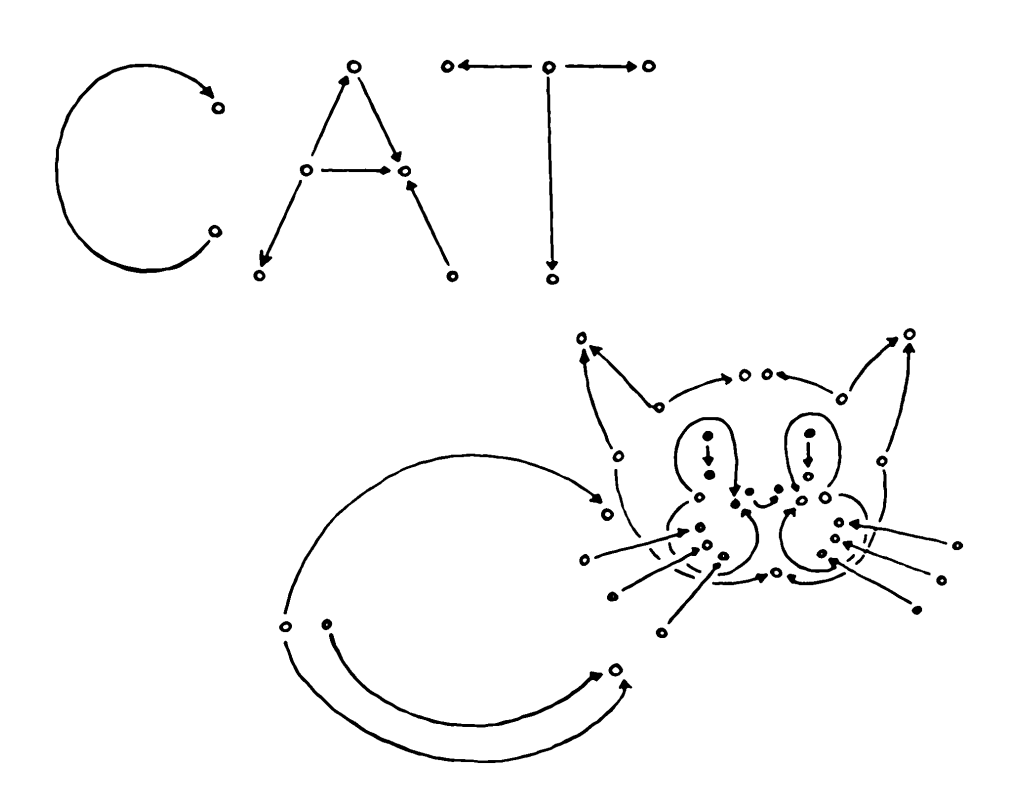
\includegraphics[scale=1.2]{cat.png}}
\hypersetup{
 pdfauthor={Jiří Adámek \& Horst Herrlich \& George E. Strecker},
 pdftitle={\aunclfamily\Huge Abstract and Concrete Categories \\ The Joy of Cats \\ 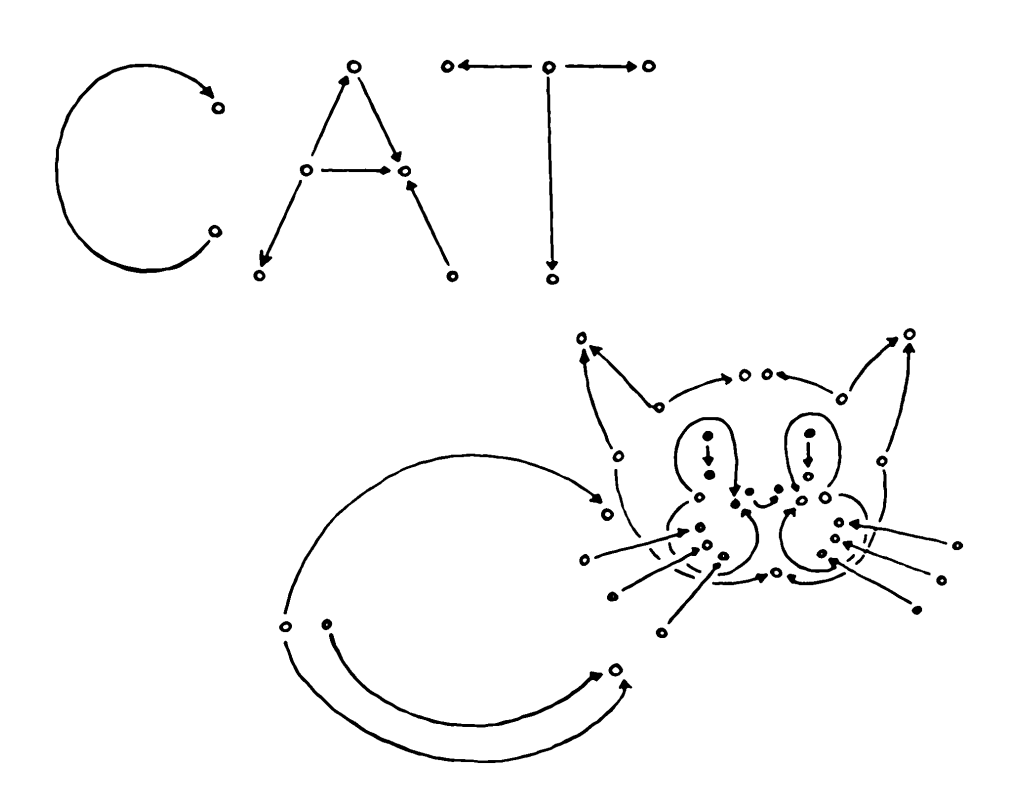
\includegraphics[scale=1.2]{cat.png}},
 pdfkeywords={},
 pdfsubject={},
 pdfcreator={Emacs 26.3 (Org mode 9.3.6)}, 
 pdflang={English}}
\begin{document}

\maketitle \clearpage
\setcounter{tocdepth}{2}
\tableofcontents \clearpage\section{Categories, Functors, and Natural Transformations}
\label{sec:org7de109f}
\subsection{Categories and Functors}
\label{sec:org28b13b6}
\subsubsection{Categories}
\label{sec:orgf070b17}
\begin{definition}[]
A \textbf{category} is a quadruple \(\bA=(\calo,\hom,id,\circ)\) consisting
\begin{enumerate}
\item a class \(\calo\), whose members are called \textbf{\(\bA\)-objects}
\item for each pair \((A,B)\) of \(\bA\)-objects, a set \(\hom(A,B)\) whose
members are called \textbf{\(\bA\)-morphisms from \(A\) to \(B\)}
\end{enumerate}
\end{definition}

\begin{examplle}[]
\begin{enumerate}
\item The following \textbf{constructs}; i.e., categories of structured sets and
structure-preserving functions between them
\begin{enumerate}
\item \(\Alg(\Omega)\) with objects all \textbf{\(\Omega\)-algebras} and morphisms all \par
\textbf{\(\Omega\)-homomorphisms} between them. Here \(\Omega=(n_i)_{i\in I}\) is a
family of natural numbers \(n_i\), indexed by a set \(I\). An
\(\Omega\)-algebra is a pair \(X,(\omega_i)_{i\in I}\) consisting of a set
\(X\) and a family of functions \(\omega_i:X^{n_i}\to X\), called \textbf{\(n_i\)-ary
operations} on \(X\). An \(\Omega\)-homomorphism \(f:(X,(\omega_i)_{i\in
         I}\to(\what{X},(\what{\omega}_i)_{i\in I})\) is a function \(f:X\to\what{X}\) for
which the diagram
\begin{center}
\begin{tikzcd}
X^{n_i}\arrow[r,"f^{n_i}"]\arrow[d,"\omega_i"']&
\what{X}^{n_i}\arrow[d,"\what{\omega}_i"]\\
X\arrow[r,"f"']&\what{X}
\end{tikzcd}
\end{center}
commutes for each \(i\in I\).
\item \textbf{\(\Sigma\)-Seq} with objects all (deterministic, sequential)
\textbf{\(\Sigma\)-acceptor}, where \(\Sigma\) is a finite set of input symbols. Objects
are quadruples \((Q,\delta,q_0,F)\) where \(Q\) is a finite set of states, 
\(\delta:\Sigma\times Q\to Q\) is a transition map, \(q_0\in Q\) is the
initial state, and \(F\subseteq Q\) is the set of final states.

A morphism \(f:(Q,\delta,q_0,F)\to(Q',\delta',q_0',F')\) (called a
\textbf{simulation}) is a function \(f:Q\to Q'\) that preserves
\begin{enumerate}
\item transitions, i.e., \(\delta'(\sigma,f(q))=f(\delta(\sigma,q))\)
\item the initial state, i.e., \(f(q_0)=q_0'\)
\item the final states, i.e., \(f[F]\subseteq F'\)
\end{enumerate}
\end{enumerate}
\item The following categories where the objects and morphisms are \emph{not}
constructed sets and structure-preserving functions:
\begin{enumerate}
\item \(\Mat\) with objects all natural numbers, and for which \(\hom(m,n)\) is
the set of all real \(m\times n\) matrices, \(id_n:n\to n\) is the unit
diagonal matrix, and composition is defined by \(A\circ B=BA\)

\item \(\Aut\) with objects all (deterministic, sequential, Moore) \textbf{automata}.
Objects are sectuples \((Q,\Sigma,Y,\delta,q_0,y)\), where \(Q\) is the set of
states, \(\Sigma\) and \(Y\) are the sets of input symbols and output symbols,
respectively, \(\delta:\Sigma\times Q\to Q\) is the transition map, 
\(q_0\in Q\) is the initial state, and \(y:Q\to Y\) is the output map.
Morphisms from an automaton \((Q,\Sigma,Y,\delta,q_0,y)\) to an automaton
\((Q',\Sigma',Y',\delta',q_0',y')\) are triples \((f_Q,f_{\Sigma},f_Y)\) of
functions satisfying the following conditions
\begin{enumerate}
\item preservation of transitions:
\(\delta'(f_{\Sigma}(\sigma),f_Q(q))=f_Q(\delta(\sigma,q))\)

\item preservation of outputs: \(f_Y(y(q))=y'(f_Q(q))\)

\item preservation of initial state: \(f_Q(q_0)=q_0'\)
\end{enumerate}
\end{enumerate}
\end{enumerate}
\end{examplle}
\subsection{The Dual Principle}
\label{sec:org9ecfb95}
\index{dual category}
\begin{definition}[]
For any category \(\bA=(\calo,\hom_{\bA},id,\circ)\) the \textbf{dual} (or \textbf{opposite})
\textbf{category of \(\bA\)} is the category
\(\bA^{\op}=(\calo,\hom_{\bA^{\op}},id,\circ^{\op})\), where
\(\hom_{\bA^{\op}}(A,B)=\hom_{\bA}(B,A)\) and \(f\circ^{\op}g=g\circ f\)
\end{definition}

Consider the property of objects \(X\) in \(\bA\):
\begin{equation*}
\calp_{\bA}(X)\equiv \textit{ For any } \bA\textit{-object } A
\textit{ there exists exactly one }
\bA\textit{-morphism } f:A\to X
\end{equation*}

Step1: In \(\calp_{\bA}(X)\) replace all occurrences of \(\bA\) by \(\bA^{\op}\),
thus obtaining the property
\begin{equation*}
\calp_{\bA^{\op}}(X)\equiv \textit{ For any } \bA^{\op}\textit{-object } A
\textit{ there exists exactly one }
\bA^{\op}\textit{-morphism } f:A\to X
\end{equation*}

Step2: Translate \(\calp_{\bA^{\op}}(X)\) into the logically equivalent
statement
\begin{equation*}
\calp_{\bA}^{\op}(X)\equiv \textit{ For any } \bA\textit{-object } A
\textit{ there exists exactly one }
\bA\textit{-morphism } f:X\to A
\end{equation*}

The \textbf{Duality Principle for Categories} states
\begin{center}
\textit{Whenever a property \(\calp\) holds for all categories,}\\
\textit{then the property \(\calp^{\op}\) holds for all categories.}
\end{center}
\section{Index}
\label{sec:orgd7312ed}
\renewcommand{\indexname}{}
\printindex
\end{document}